\sectionquestion{S22 TA Questions Go Here!}

\begin{parts}
    \part Inspired by the homework question saying you should not train a logistic regression model without regularization, you decide to add a regularizer to your Homework 4 model implementation. Recall that for a design matrix $\Xv \in \mathbb{R}^{N \times (M+1)}$, labels $\yv \in \mathbb{R}^{N}$, and parameter vector $\thetav \in \mathbb{R}^{M+1}$ (bias folded in), the SGD update rule was
    \[
    \thetav \leftarrow \thetav + \alpha \xv^{\left(i\right)} \left[y^{(i)}-\frac{e^{\thetav^T\xv^{\left(i\right)}}}{1+e^{\thetav^T\xv^{\left(i\right)}}}\right],
    \]
    where $\alpha >0$ is the learning rate. You include a regularization term and change this to
    \[
    \thetav \leftarrow \thetav - \alpha \lambda \thetav + \alpha \xv^{\left(i\right)} \left[y^{(i)}-\frac{e^{\thetav^T\xv^{\left(i\right)}}}{1+e^{\thetav^T\xv^{\left(i\right)}}}\right],
    \]
    where $\lambda > 0$ is a hyperparameter.
    
    \begin{subparts}
        \subpart[1] \textbf{Select one:} What regularization is applied to $\thetav$?
            \begin{checkboxes}
             \choice $\ell_0$ regularization
             \choice $\ell_1$ regularization
             \choice $\ell_2$ regularization
            \end{checkboxes}
            \begin{soln}
            C \\
            (if we have a question directly related to the SGD update rule, we can change this to give the new $J(\thetav)$ with $+\frac{\lambda}{2}\|\thetav\|_2^2$ added and make students derive the new update rule based on that instead) 
            \end{soln}

        \subpart[2] \textbf{Short answer:} Now you test this new update rule with a perfectly linearly separable dataset, but the performance is terrible no matter what hyperparameters you choose! Your friend tells you this is because you made a mistake when adding the regularization term. What is this mistake, and what can you infer about the linear separator of this dataset?
        
            \fillwithlines{4em}
            \begin{soln}
            Mistake: The bias term is regularized. \\
            Dataset: The linear separator of the dataset has a nonzero intercept.
            \end{soln}
    \end{subparts}

    \begin{qauthor}
    Hayden Kim

    Learning Objectives: \\
    3d. Implement logistic regression for binary or multiclass classification \\
    4d. Add a regularizer to an existing objective in order to combat overfitting \\
    4e. Explain why we should not regularize the bias term
    
    Based on an actual bug I had
    
    Comments from Brynn: I like part a. Part b is a little tricky, but its a good question.
    \end{qauthor}
    
    
    
    \part[1] \textbf{Select all that apply:} Which of the following functions are convex? 
    {%
    \checkboxchar{$\Box$} \checkedchar{$\blacksquare$} % change checkbox style locally
    \begin{checkboxes}
     \choice $f(x) = - \frac{1}{1+e^{-x}}$
     \choice $f(x) = - log \left(\frac{1}{1+e^{-x}}\right)$
     \choice $f(x) = |x|$
     \choice $f(x) = x^4$
     \choice $f(x) = -\log\left(\sin x\right), x \in [0, \pi]$
    \end{checkboxes}
    }
    \begin{soln}
    B, C, D, E
    \end{soln}
    \begin{qauthor}
    Prasoon Varshney
    
    Learning Objective: 
    Distinguish between convex, concave, and nonconvex functions
    
    Comments from Brynn: Out of scope of an exam. Not obvious if log(sin(x)) is convex or not
    \end{qauthor}
    
\part[2] \textbf{Pseudocode:} Now we will revisit a familiar optimization method using pseudocode. Consider a model with parameter $\thetav \in \mathbb{R}^M$ being trained with a design matrix $\Xv \in \mathbb{R}^{N \times M}$ and labels $\yv \in \mathbb{R}^N$. Say we update $\thetav$ using the objective function $J(\thetav|\Xv, \yv) = \frac{1}{N} \sum_{i=1}^N J^{(i)}(\thetav|\xv^{(i)}, y^{(i)}) \in \mathbb{R}$.  Using this, complete the pseudocode for stochastic gradient descent that samples \textit{without} replacement.
\begin{lstlisting}[language=Python,escapechar=@]
def dJ(theta, X, y, i):
    (omitted)  # Returns @$\partial J^{(i)}(\thetav|\xv^{(i)}, y^{(i)})/\partial\thetav$@
    # You may call this function in your pseudocode.

def SGD(theta, X, y, learning_rate):
    for epoch in range(num_epoch):
        indices = shuffle(range(len(X)))
        for i in indices:
            @\underline{$~~~$\textbf{Complete this section with the update rule}$~~~$}@
    return theta  # return the updated theta
\end{lstlisting}

    \begin{tcolorbox}[fit,height=3cm, width=15cm, blank, borderline={1pt}{-2pt}]
    %solution
    \end{tcolorbox}
    \begin{soln}
   theta -= learning\_rate * dJ(theta, X, y, i)
    \end{soln}
    \begin{qauthor}
   written by Hayden for the homework, stolen by Tori for the exam. Learning objective addressed: 
b. Implement learning for Linear Regression using three optimization techniques: (1)
closed form, (2) gradient descent, (3) stochastic gradient descent. Taken directly from HW4.
    
    
    Comments from Brynn: They could use the answers from Q1 to solve this. So if we use this, we would not use the first question.
    \end{qauthor}
    
\part[2] \textbf{Numerical answer:} Recall that for logistic regression, we normally minimize over the negative conditional \textit{log} likelihood. Late one night, Neural, a 10-601 student, is doing their homework and they forget to copy the $\log$ from the slides and instead begin attempting to minimize over the negative conditional likelihood $J(\theta) = \prod_{i =1}^N p_{\theta}(y^{(i)} | x^{(i)}) $
 What are some issues Neural may run into when implementing logistic regression with this objective function?\\
\begin{tcolorbox}[fit,height=2cm, width=15cm, blank, borderline={1pt}{-2pt}]
    %solution
    \end{tcolorbox}
    \begin{soln}
    Input solution here.
    \end{soln}

  
    \begin{qauthor}
    Input (1) author name, (2) learning objective addressed, and (3) source if  adapting/reusing a question.
    
    Comments from Brynn: No solution given. But I think the question is implying this would set everything to zero?
    \end{qauthor}
    
    
\part[2] Consider the following prediction function $p(y = 1 \mid \thetav_1, \thetav_2, \x)$, where $\thetav_1 \in \mathbb{R}^d$ and $\thetav_2, \x \in \mathbb{R}^d$: 

$$p(y = 1 \mid \thetav_1, \thetav_2, \x) = \frac{\exp(\thetav_1^T\x)}{\exp(\thetav_1^T\x) + \exp(\thetav_2^T\x)} $$

What is the Bayes Optimal classifier for this probabilistic model? Write your answer as an inequality in terms of $\thetav_1, \thetav_2, \text{ and } \x$. You should not have a probability in your final answer. Assume we break ties in favor of $y = 1$.

\begin{tcolorbox}[fit,height=5.5cm, width=15cm, blank, borderline={1pt}{-2pt}]
    %solution
    \begin{soln}
    \begin{align*}
        & p(y = 1 \mid \thetav_1, \thetav_2, \x)  \geq p(y = 0 \mid \thetav_1, \thetav_2, \x) \\
        & \implies y = 1 \text{ iff } \frac{\exp(\thetav_1^T\x)}{\exp(\thetav_1^T\x) + \exp(\thetav_2^T\x)} \geq \frac{\exp(\thetav_2^T\x)}{\exp(\thetav_1^T\x) + \exp(\thetav_2^T\x)} \\
        & \implies y = 1 \text{ iff } \frac{\exp(\thetav_1^T\x)}{\exp(\thetav_2^Tx)} \geq 1
    \end{align*}
    \end{soln}
\end{tcolorbox}

\begin{qauthor}
Sana, 3b. (Logistic Regression) Given a discriminative probabilistic model, derive the conditional log-likelihood, its gradient, and the corresponding Bayes Classifier, 1 point for Bayes optimal classifier assumption, 1 point for correct answer.

Comments from Brynn: This is a good question, but maybe a bit hard for the exam?

Sana: then I'm glad I wrote version 2 below! no changes here since I had version 2 ready to go.

Abhi: I like this, but you might want to more formally define $h$ in terms of the conditional probability, since you reference $h$. I also think that you'll just get a lot of not simplified answers or issues like last semester with "in terms of" being interpreted weirdly.

Sana: +1 to the "in terms of" comment. I think I would recommend using version 2 below. Also oops, that was leftovers from when I was iterating on a previous version of this question. Thanks! I think I'll get rid of it since it's an extra definition students don't need.
\end{qauthor}


\part[2]
Consider the following computation graph of a neural network, we have $\xv^* = [x_1, x_2]^T$ as our original input. We add a bias term and make $\xv \in \mathbb{R}^3$. Similarly, we add a bias term to $\zv^*$ in the graph and make it $\zv$. Given $\alphav$ and $\betav$ are weight matrices, $\yv$ is the true label, and $J$ is the unknown loss function.

\begin{figure}[ht]
    \def\distH{2.5cm}
    \def\distHTwo{0.1cm}
    \def\distHThree{0.3cm}
    \def\distV{1cm}
    \def\distVTwo{0.3cm}
    \centering
    \begin{tikzpicture}[
        > = stealth, % arrow head style
        shorten > = 0pt, % don't touch arrow head to node
        auto,
        % node distance = 2.5cm, % distance between nodes
        thick % line style
    ]\footnotesize
    \tikzstyle{every state}=[
        draw = black,
        thick,
        fill = white,
        minimum size = 0.8cm,
        shape = rectangle
    ]
    
    \node[state] (X) {$\xv$};
    \node[state] (b) [label=above:{$\bv$}, right = \distV of X ] {$\alphav\xv$};
    \node[state] (z) [label=above:{$\zv^*$}, right = \distV of b] {$\sigma (\bv)$};
    \node[state] (y_hat)
    [label=above:{$\hat{\yv}$}, right = \distV of z ] {$\betav\zv$};
    \node[state] (l)
    [label=above:{$l$}, right = \distV of y_hat] {$J(\hat{\yv}, \yv)$};
    \node[state] (alpha) [below = \distVTwo of b] {$\alphav$};
    \node[state] (beta) [below = \distVTwo of y_hat] {$\betav$};
    \node[state] (y) [below = \distVTwo of l] {$\yv$};
    
    \path[->] (X) edge node {} (b);
    \path[->] (b) edge node {} (z);
    \path[->] (z) edge node {} (y_hat);
    \path[->] (y_hat) edge node {} (l);
    \path[->] (alpha) edge node {} (b);
    \path[->] (beta) edge node {} (y_hat);
    \path[->] (y) edge node {} (l);
    \end{tikzpicture}
    \caption{A computation graph}
    \label{fig:backprop_graph}
    \end{figure}

Choose some elements from the given partial derivatives pool (be aware that some of them are not legitimate/necessary for this problem):\\
\begin{align*}
    \frac{\partial{l}}{\partial{\hat{\yv}}},
    \frac{\partial{l}}{\partial{\zv}},
    \frac{\partial{l}}{\partial{\zv^*}}, \frac{\partial{l}}{\partial{\betav}}, 
    \frac{\partial{\hat{\yv}}}{\partial{\betav}}, 
    \frac{\partial{\hat{\yv}}}{\partial{\zv}}, 
    \frac{\partial{\betav}}{\partial{\zv}},
    \frac{\partial{\zv}}{\partial{\bv}},
    \frac{\partial{\zv^*}}{\partial{\bv}},
    \frac{\partial{\bv}}{\partial{\alphav}}
\end{align*}
and write out the formula for computing $\frac{\partial{l}}{\partial{\alphav}} $ in backward propagation.

\begin{tcolorbox}[fit,height=3cm, width=15cm, blank, borderline={1pt}{-2pt}]

\end{tcolorbox}
\begin{soln}
    $\frac{\partial{l}}{\partial{\alpha}} = \frac{\partial{l}}{\partial{z^*}}\frac{\partial{z^*}}{\partial{b}}\frac{\partial{b}}{\partial{\alpha}}$
\end{soln}
\begin{qauthor}
   Shelly.
   Learning Objectives: Carry out the backpropagation on an arbitrary computation graph. Inspired by HW5 and recitation problem to address the bias term during backprop.
   
   Comments from Brynn: Vectors should either have the line over them or be in bold. E.g. for dl/dz should z be in vector form? Also, I like that this makes the distinction between z* and z. I think this is what separates a true understanding of backprop in this question
   
   Update: Change all the vectors and partial derivatives with vectors to bold form.
\end{qauthor}

\part Choose what kinds of models should be used in each scenario.
    \begin{subparts}
    \subpart[1] You’ve finished a few pages of a new novel and tried to guess what will be the first sentence in the next page.
    \begin{checkboxes}
     \choice Generative Model
     \choice Discriminative Model
     \choice Both models
     \choice None of the above
    \end{checkboxes}
    \begin{soln}
    A. Sampling from the previous chapter and assign a probability to generate a sequence of words.
    \end{soln}
    \subpart[1] You’ve finished 80\% of this novel. When you read halfway through a new chapter, you are trying to guess what will be the mood of the entire chapter.
    \begin{checkboxes}
     \choice Generative Model
     \choice Discriminative Model
     \choice Both models
     \choice None of the above
    \end{checkboxes}
    \begin{soln}
    C. Sampling the next half of the chapter with a generative model. Using previous chapters as training set and output the prediction of mood with a discriminative model.
    \end{soln}
    \subpart[1] You finished the book and want to find out how others like it. Before you search through your favorite book rating websites that you’ve used for years, you try to guess how many stars it would be rated out of a total of five stars (there's no half stars).
    \begin{checkboxes}
     \choice Generative Model
     \choice Discriminative Model
     \choice Both models
     \choice None of the above
    \end{checkboxes}
    \end{subparts}
    \begin{soln}
    B. Use discriminative model to solve this classification problem.
    \end{soln}
    \begin{qauthor}
       Shelly.
       Learning Objectives: Describe the tradeoffs of generative vs. discriminative models.
       
       Comments from Brynn: I like thought process required for this one, I think it makes an important distinction. But I think it is a little too abstract for the exam. It would be hard to grade.
       
       Update: Get rid of the explanation part. Hopefully it's easier to grade right now.
    \end{qauthor}


\part[1] \textbf{True or False:} Biological neural networks are generally much smaller than artificial neural networks (in neuron count).
    \begin{checkboxes}
     \choice True
     \choice False
    \end{checkboxes}
    \begin{soln}
    False
    \end{soln}
    \begin{qauthor}
    Abhi, S22 Deep Learning 1.a: Explain the biological motivations for a neural network
    
    Brynn's Comments: I think this is a bit out of scope. 
    
    Comments from Abhi: Me too.
    
    Sana: weird side note do we really even know how the human brain works? Can we really draw an equivalence or comparison between artificial and biological neural networks?
    
    Abhi: Great point! I'm not sure we can test this learning objective without asking them to regurgitate the single relevant slide via their cheat sheets.
    
    Sana: +1!
    \end{qauthor}

    


\part Given that the error for linear regression has a normal distribution, show that minimizing squared is equivalent to maximizing conditional likelihood.
\[
        P(\epsilon^{(i)}) = \frac{1}{\sqrt{2\pi}\sigma} exp(-\frac{(\epsilon^{(i)})^2}{2\sigma^2})
    \]
    \begin{tcolorbox}[fit,height=3cm, width=15cm, blank, borderline={1pt}{-2pt}]

\end{tcolorbox}
    \begin{soln}
    $P(x_1 .. x_n) = \prod_{i=1}^{n} \frac{1}{\sqrt{2\pi}\sigma} exp(-\frac{(\epsilon^{(i)})^2}{2\sigma^2})$ \\
    log(likelihood) = nlog$\frac{1}{\sqrt{2\pi}\sigma}$ - $\sum_{i=1}^{n}-(\frac{(\epsilon^{(i)})^2}{2\sigma^2})$ \\
    by dropping the constants, you can see that -log(likelihood) = $\sum_{i=1}^{n} (\epsilon^{(i)})^2$ = squared error \\
    \end{soln}
    \begin{qauthor}
    Rita, Generative Models 1.g: For linear regression, show that the parameters which minimize squared error are equivalent to those that maximize conditional likelihood
    
    Brynn's Comments: We should state that the eqn is the Gaussian. We should state what epsilon is. 

    \end{qauthor}
    
    \part[3] \textbf{Drawing:} For the following neural network, draw the corresponding computational graph. Assume that all hidden units use the sigmoid function ($\sigma$) as the activation function and that the loss is mean squared error. Provide the shape of all parameters defined in the computational graph. Assume the weights for the first layer and second layers are respectively the matrices $\alphav$ and $\betav$ and assume no weights used from $b_k$ to $\hat{y}$. 

\begin{figure}[h]
    \def\distH{2cm}
    \def\distHTwo{0.1cm}
    \def\distHThree{0.3cm}
    \def\distV{0.3cm}
    \def\distVTwo{0.1cm}
    \centering
    \begin{tikzpicture}[
        > = stealth, % arrow head style
        shorten > = 0pt, % don't touch arrow head to node
        auto,
        % node distance = 2.5cm, % distance between nodes
        thick % line style
    ]\footnotesize
    \tikzstyle{every state}=[
        draw = black,
        thick,
        fill = white,
        minimum size = 0.8cm,
    ]
    \node[state] (X1) {$x_1$};
    \node[state] (X2) [below = \distV of X1] {$x_2$};
    \node[state] (X3) [below = \distV of X2] {$x_3$};
    \node[state] (X4) [below = \distV of X3] {$x_4$};
    \node[state] (X5) [below = \distV of X4] {$x_5$};
    \node[state] (A1) [below right = \distVTwo and \distH of X1] {$a_1$};
    \node[state] (A2) [below = \distV of A1] {$a_2$};
    \node[state] (A3) [below = \distV of A2] {$a_3$};
    \node[state] (A4) [below = \distV of A3] {$a_4$};
    \node[state] (B1) [below right = \distVTwo and \distH of A1] {$b_1$};
    \node[state] (B2) [below = \distV of B1] {$b_2$};
    \node[state] (B3) [below = \distV of B2] {$b_3$};
    \node[state] (y_hat) [right = \distHThree of B2] {$\hat{y}$};

    \path[->] (X1) edge node {} (A1);
    \path[->] (X1) edge node {} (A2);
    \path[->] (X1) edge node {} (A3);
    \path[->] (X1) edge node {} (A4);
    \path[->] (X2) edge node {} (A1);
    \path[->] (X2) edge node {} (A2);
    \path[->] (X2) edge node {} (A3);
    \path[->] (X2) edge node {} (A4);
    \path[->] (X3) edge node {} (A1);
    \path[->] (X3) edge node {} (A2);
    \path[->] (X3) edge node {} (A3);
    \path[->] (X3) edge node {} (A4);
    \path[->] (X4) edge node {} (A1);
    \path[->] (X4) edge node {} (A2);
    \path[->] (X4) edge node {} (A3);
    \path[->] (X4) edge node {} (A4);
    \path[->] (X5) edge node {} (A1);
    \path[->] (X5) edge node {} (A2);
    \path[->] (X5) edge node {} (A3);
    \path[->] (X5) edge node {} (A4);
    \path[->] (A1) edge node {} (B1);
    \path[->] (A1) edge node {} (B2);
    \path[->] (A1) edge node {} (B3);
    \path[->] (A2) edge node {} (B1);
    \path[->] (A2) edge node {} (B2);
    \path[->] (A2) edge node {} (B3);
    \path[->] (A3) edge node {} (B1);
    \path[->] (A3) edge node {} (B2);
    \path[->] (A3) edge node {} (B3);
    \path[->] (A4) edge node {} (B1);
    \path[->] (A4) edge node {} (B2);
    \path[->] (A4) edge node {} (B3);
    \path[->] (B1) edge node {} (y_hat);
    \path[->] (B2) edge node {} (y_hat);
    \path[->] (B3) edge node {} (y_hat);
    \end{tikzpicture}
\end{figure}

    \begin{tcolorbox}[fit,height=6cm, width=15cm, blank, borderline={1pt}{-2pt}]
    %solution
    \end{tcolorbox}
    \begin{soln}
    \begin{figure}[h]
    \def\distH{2.5cm}
    \def\distHTwo{0.1cm}
    \def\distHThree{0.3cm}
    \def\distV{1cm}
    \def\distVTwo{0.3cm}
    \centering
    \begin{tikzpicture}[
        > = stealth, % arrow head style
        shorten > = 0pt, % don't touch arrow head to node
        auto,
        % node distance = 2.5cm, % distance between nodes
        thick % line style
    ]\footnotesize
    \tikzstyle{every state}=[
        draw = black,
        thick,
        fill = white,
        minimum size = 0.8cm,
        shape = rectangle
    ]
    \node[state] (X) {$\Vec{x}$};
    \node[state] (a_temp) [label=above:{$\Vec{a'}$}, right = \distV of X ] {$\alphav\Vec{x} + \alphav_{0}$};
    \node[state] (a) [label=above:{$\Vec{a}$}, right = \distV of a_temp] {$\sigma (\Vec{a'})$};
    \node[state] (b_temp) [label=above:{$\Vec{b'}$}, right = \distV of a] {$\betav \Vec{a} + \betav_{0}$};
    \node[state] (b) [label=above:{$\Vec{b}$}, right = \distV of b_temp] {$\sigma (\Vec{b'})$};
    \node[state] (y_hat) [label=above:{$\hat{y}$}, right = \distV of b] {$\sum_{i=1}^{3} b_i$};
    \node[state] (loss) [label=above:{$l$}, right = \distV of y_hat] {$(\hat{y}-y)^2$};
    \node[state] (alpha) [below = \distVTwo of a_temp] {$\alphav$};
    \node[state] (alpha_0) [left = \distVTwo of alpha] {$\alphav_{0}$};
    
    \node[state] (beta) [below = \distVTwo of b_temp] {$\betav$};
    \node[state] (beta_0) [left = \distVTwo of beta] {$\betav_{0}$};
    \node[state] (y) [below = \distVTwo of loss] {$y$};
    
    \path[->] (X) edge node {} (a_temp);
    \path[->] (a_temp) edge node {} (a);
    \path[->] (a) edge node {} (b_temp);
    \path[->] (b_temp) edge node {} (b);
    \path[->] (b) edge node {} (y_hat);
    \path[->] (y_hat) edge node {} (loss);
    \path[->] (alpha) edge node {} (a_temp);
    \path[->] (alpha_0) edge node {} (a_temp);
    \path[->] (beta) edge node {} (b_temp);
    \path[->] (beta_0) edge node {} (b_temp);
    \path[->] (y) edge node {} (loss);
    \end{tikzpicture}
\end{figure}

$$\alphav \in \mathbb{R}^{4 \times 5} \;\;\;\; \alphav_{0} \in \mathbb{R}^{4} \;\;\;\; \betav \in \mathbb{R}^{3 \times 4} \;\;\;\; \betav_{0} \in \mathbb{R}^{3}$$
    \end{soln}
    \begin{qauthor}
    Author: Udai\\
    Objective: Construct a computation graph for a neural network, identifying all the given and intermediate quantities that are relevant
    
    Bryn's comments: I like this question, but it will be a pain to grade. But this may be fine as it is an important concept.
    \end{qauthor}
    



\part[2] \textbf{Numerical answer:} Suppose Yumeko wishes to model some data according to the following distribution:
    \[
        f(x) = \begin{cases}
        \lambda x^{\lambda - 1} & 0 < x < 1 \\
        0 & \text{otherwise}
        \end{cases}
    \]
    If she observes the single data point $x^{(1)} = \frac{1}{\sqrt{e}}$, what is the MLE estimate $\hat{\lambda}$?
    \begin{tcolorbox}[fit,height=1cm, width=2cm, blank, borderline={1pt}{-2pt}]
    %solution
    \end{tcolorbox}
    \begin{soln}
    $\ell(\lambda; x^{(1)}) = \log \lambda - \frac{1}{2}(\lambda - 1)$ \\
    $\frac{\partial \ell}{\partial \lambda} = \frac{1}{\lambda} - \frac{1}{2} = 0$ \\
    $\hat{\lambda} = 2$ \\
    \end{soln}
    \begin{qauthor}
    Alex\\
    Derive the MLE or MAP parameters of a simple model in closed form
    
    Brynn's Comments: We should specify that e is the exponential function
    
    Do we want to tell people to use natural log? Or add a hint that they can use any log base they choose? I am worried the equation will be a nightmare to grade otherwise, but do not want to over simplify the question
    \end{qauthor}


\part[3] One of the assumptions made in linear regression is that each observation, $y_i$, is independent and identically Gaussian-distributed for a given input, $x_i$, $\forall i \in \{1...K\}$. With this assumption, we can write the model with a probabilistic formulation, $$y_i \mid x_i \sim N(w x_i, \sigma^2).$$ 
Note that for simplicity, we assume just one input to the model and no bias term, ie: we predict $\hat{y}_i = w x_i$. Given this setup, find the maximum likelihood estimate of the $w$ parameter for the linear model above. To help you get started, we have written out the linear regression objective function as the product of conditional probabilities:

$$J(w) = \prod_{i=1}^K \frac{1}{\sigma \sqrt{2\pi}} e^{-\frac{1}{2} \left(\frac{y_i-w x_i}{\sigma}\right)^2}$$

\begin{tcolorbox}[fit,height=7cm, width=15cm, blank, borderline={1pt}{-2pt}]
    %solution
    \begin{soln}
    \begin{align*}
        0 = & \frac{\partial}{\partial w} \log \prod_{i=1}^K \frac{1}{\sigma \sqrt{2\pi}} e^{-\frac{1}{2} \left(\frac{y_i-w x_i}{\sigma}\right)^2} \\
        0 = & \sum_{i=1}^K \left[ \frac{y_i-w x_i}{\sigma} \right] x_i \\
        w \sum_{i=1}^K x_i^2 = & \sum_{i=1}^K y_i x_i \\
        w = & \frac{\sum_{i=1}^K y_i x_i}{\sum_{i=1}^K x_i^2}
    \end{align*}
    \end{soln}
\end{tcolorbox}

\begin{qauthor}
Sana, 3f. (Logistic Regression) For linear regression, show that the parameters which minimize squared error are equivalent to those that maximize conditional likelihood; also covers 3a. (Logistic Regression) Apply the principle of maximum likelihood estimation (MLE) to learn the parameters of a probabilistic model, 1 point to take a log, 1 point to take a derivative and set it to 0, 1 point for the correct answer.

Comments from Brynn: Why do we use beta instead of theta or w? This may throw some people off.

Sana: you can take the girl out of the stats major but you can't take the stats major out of the girl lmao, changed $\beta$ to $w$! also @Matt this didn't hit me before but we have similar questions to this in HW6, use with discretion!

Abhi: Echoing the comment about HW6. I'm also unsure how confusing it would be for students that we say both $y_i \mid x_i \sim N(w x_i, \sigma^2)$ and $y_i = w x_i$. I could see some students dropping the variance term not because it doesn't apply to the derivative but because we gave them that second equation, which would give them the correct answer with incorrect derivation (both annoying to grade and something students might complain about in regrades).

Sana: that's my bad, one of those was supposed to be $\hat{y}_i$, good catch!
\end{qauthor}

    
\part
\begin{subparts}
    \subpart[1] \textbf{Select one:} Which of the following is a valid approximation to use for a finite difference check of the gradient of the function $f$ at $x$? Assume $\epsilon$ is a small value.
    \begin{checkboxes}
     \choice $\dfrac{f(x + \epsilon) - f(x - \epsilon)}{\epsilon^2}$
     \choice $\dfrac{f(x + \epsilon) - f(x - \epsilon)}{\epsilon}$
     \choice $\dfrac{f(x + \epsilon) - f(x)}{\epsilon}$
    \end{checkboxes}

    \begin{soln}
    C.
    \end{soln}
    
    \subpart[1] Suppose we have $f(0.999) = 0.101$, $f(1.000) = 0.301$, $f(1.001) = 0.601$. Estimate the gradient of $f$ at $1.000$ with $\epsilon = 0.001$ using the valid method from the previous part.
    
    \begin{tcolorbox}[fit,height=1cm, width=2cm, blank, borderline={1pt}{-2pt}]
    %solution
    \end{tcolorbox}
    \begin{soln}
    $(.601-.301)/(.001) = 300$
    \end{soln}
    \begin{qauthor}
    Abhi, S22 Deep Learning 2.g: Use the finite difference method to evaluate the gradient of a function
    
    Comments from Brynn: Are we expecting them to memorize the finite difference method? This may be a little bit difficult. 
    
    Comments from Abhi: I guess this ends up being more of a prereq question? Testing what is a "valid" derivative approximation.
    
    Sana: other dangers of this question: it could just be a test of whether you wrote down the finite difference method on your cheat sheet. Maybe we could make them do an example?
    
    Abhi: I think that Matt presents one of these in class but not the other (for the correct answers). Should we remove the one that's likely to appear on cheat sheets and replace it with something else? Example also sounds worth, probably for an extra point.
    
    Sana: That's a valid solution too. I'd be good with either!
    
    Abhi: I'll change it to select one, remove the one that appears on lecture slides, and then add an example.
    
    Sana: All of the above lmao- that works!
    
    Abhi: Example completed, worth 1 point only achievable if they get the first part correct.
    \end{qauthor}
    
\end{subparts}



\part[2] \textbf{Select all that apply:} Tired of using the same architecture over and over, Neural the Narwhal decides to create a new type of linear layer where each neuron maps to exactly one neuron in the next layer. Select all of the following that are true when using this layer in place of a linear layer in a neural network architecture.
    {%
    \checkboxchar{$\Box$} \checkedchar{$\blacksquare$} % change checkbox style locally
    \begin{checkboxes}
     \choice The neurons in a hidden layer are more likely to learn different feature representations
     \choice The network will be slower to train because the linear layer operation cannot be vectorized
     \choice The network learns fewer parameters
     \choice The network may be able to learn more complex functions than before
     \choice The network may be more prone to overfitting
     \choice None of the above
    \end{checkboxes}
    }
    \begin{soln}
    A, C. A is true because the hidden layer neurons now have exclusive inputs of different parts of the input, so it is very hard to learn the same features. B is false because the easy impl is just zeroing values in the linear matrix, which makes it still vectorized. C is true because the network is losing parameters while maintaining the same general architecture (see note on implementation in B). D is false because C is true. E is false because D is false.
    \end{soln}
    \begin{qauthor}
    Abhi, S22 Deep Learning 1.e: Identify (some of) the options available when designing the architecture of a neural network
    
    Brynn's Comments: This may be a bit difficult if students have not had to think about dropout too much before. 
    
    Comments from Abhi: I don't think this necessarily references dropout? This gets at the idea of the difference between the connections in the linear layer and an activation layer in the, e.g., HW5 network, where we have $\mathbf{z} = \sigma (\mathbf{a})$ as a derivative they need to compute (which ends up being a diagonal matrix). The idea would be that they recognize features can no longer be combinations of other features.
    
    Sana: I agree with Abhi here- I see how this one can make students stop and think, but I think that has value in this case. One way we might be able to help them along is by saying (for options C and D) "the network learns fewer parameters, which may limit its ability to learn functions that are as complex as before. however, this may reduce the risk of overfitting" and "the network learns fewer parameters, which may increase its ability to learn functions that are as complex as before. however, this may increase the risk of overfitting"- might be too wordy though, there's probably a better way to do this.
    
    Abhi: Updated based on the above feedback to split "fewer parameters," "ability to learn complex functions," and "risk of overfitting" into 3 separate answer choices. Also wanted to note that this should not relate too much to dropout because it's a permanent architecture change instead of a randomly sampled mask.
    
    Sana: echoing last comment above. This question looks good to me!
    \end{qauthor}



\part 
    Neural the Narwhal has loved learning about different ML models, but he's confused about when and why we use MLE vs. MAP. 
    %In the questions below, assume $\mathbf{X}$ is some dataset and $\theta$ are model parameters.
    
    \begin{subparts}
        \subpart[1]
            Given $p(\mathbf{X}\mid \theta)$, can we perform MLE, MAP, or both?
            
            \begin{checkboxes}
                \choice MLE only
                \choice MAP only
                \choice Both MLE and MAP
                \choice Neither
            \end{checkboxes}
            \begin{soln}
                A (MLE only)
            \end{soln}
            

        \subpart[1]
            Given $p(\theta\mid \mathbf{X})$, can we perform MLE, MAP, or both?
            
            \begin{checkboxes}
                \choice MLE only
                \choice MAP only
                \choice Both MLE and MAP
                \choice Neither
            \end{checkboxes}
            \begin{soln}
                D (neither/none)
            \end{soln}


        \subpart[1]
            Given $p(\theta)$ and $p(\mathbf{X}\mid \theta)$, can we perform MLE, MAP, or both?
            
            \begin{checkboxes}
                \choice MLE only
                \choice MAP only
                \choice Both MLE and MAP
                \choice Neither
            \end{checkboxes}
            \begin{soln}
                C (both MLE and MAP)
            \end{soln}


        \subpart[1]
            Given $p(\theta, \mathbf{X})$, can we perform MLE, MAP, or both?
            
            \begin{checkboxes}
                \choice MLE only
                \choice MAP only
                \choice Both MLE and MAP
                \choice Neither
            \end{checkboxes}
            \begin{soln}
                C (both MLE and MAP)
            \end{soln}


        \subpart[1]
            \textbf{True or false:} Whenever we can do MLE, we can also do MAP.
            
            \begin{checkboxes}
                \choice True
                \choice False
            \end{checkboxes}
            \begin{soln}
                B (False)
            \end{soln}


        \subpart[1]
            \textbf{True or false:} Whenever we can do MAP, we can also do MLE.
            
            \begin{checkboxes}
                \choice True
                \choice False
            \end{checkboxes}
            \begin{soln}
                A (True)
            \end{soln}

    \end{subparts}
    
    
    \begin{qauthor}
       Chu. Learning objectives: MLE and MAP 2c State the principle of maximum likelihood estimation and explain what it tries to accomplish; Naive Bayes 3d Motivate the need for MAP estimation through the deficiencies of MLE
    \end{qauthor}


\part 
    Mininet is a neural network with a single hidden layer and one output neuron. The main difference between Mininet and a fully connected neural network is that, in Mininet, each hidden unit $v_i$ connects only to the corresponding $x_i$. More specifically, given an input $\xv\in\mathbb{R}^n$, each of the $n$ hidden units computes its activation $z_i$ as
    
    $$a_i = w_i x_i + b_i$$
    $$z_i = f(a_i)$$
    
    where $w_i\in\mathbb{R}$ is the weight, $b_i\in\mathbb{R}$ is the bias, and $f:\mathbb{R}\rightarrow \mathbb{R}$ is the activation function.
    
    Then, the final output neuron computes
    
    $$a_{out} = \mathbf{w}_{out}^T \mathbf{z} + b_{out}$$
    $$z_{out} = g(a_{out})$$
    
    where $\mathbf{z}\in\mathbb{R}^n$ is the vector containing the hidden units' activations, $\mathbf{w}_{out}\in\mathbb{R}^n$ is the weight vector, and $b_{out}\in\mathbb{R}$ is the bias term.
    
    A diagram of Mininet is provided below.
    
    % NOTE: Much credit for the code below goes to Abbey and Udai -- I used mostly the same code 
    % that they used in their graphs because I don't know how to do these tikzstyle graphs.
    \begin{figure}[H]
        \def\distH{3.5cm}
        \def\distHTwo{0.1cm}
        \def\distHThree{0.3cm}
        \def\distV{0.6cm}
        \def\distVTwo{0.3cm}
        \centering
        \begin{tikzpicture}[
            > = stealth, % arrow head style
            shorten > = 0pt, % don't touch arrow head to node
            auto,
            % node distance = 2.5cm, % distance between nodes
            thick % line style
        ]\footnotesize
        \tikzstyle{every state}=[
            draw = black,
            thick,
            fill = white,
            minimum size = 0.8cm,
        ]
        \node[state] (X1)                        {$x_1$};
        \node[state] (X2) [below = \distV of X1] {$x_2$};
        \node[state] (X3) [below = \distV of X2] {$x_3$};
        \node[state] (X4) [below = \distV of X3] {$x_4$};
        
        \node[state] (V1) [right = \distH of X1] {$z_1$};
        \node[state] (V2) [right = \distH of X2] {$z_2$};
        \node[state] (V3) [right = \distH of X3] {$z_3$};
        \node[state] (V4) [right = \distH of X4] {$z_4$};
        
        \node[state] (Vo) [above right = \distVTwo and \distH of V3] {$z_{out}$};
    
        \path[->] (X1) edge node {} (V1);
        \path[->] (X2) edge node {} (V2);
        \path[->] (X3) edge node {} (V3);
        \path[->] (X4) edge node {} (V4);
        
        % \path[->] (V1) edge node {$f(w_1 x_1 + b_1)$} (Vo);
        % \path[->] (V2) edge node {$f(w_2 x_2 + b_2)$} (Vo);
        % \path[->] (V3) edge node {$f(w_3 x_3 + b_3)$} (Vo);
        % \path[->] (V4) edge node {$f(w_4 x_4 + b_4)$} (Vo);
        % \draw[->] (Vo) --++(0:3.5cm) node[above,midway] {$g(\mathbf{w}_{out}^T \mathbf{z} + b_{out})$};
        
        \path[->] (V1) edge  (Vo);
        \path[->] (V2) edge (Vo);
        \path[->] (V3) edge (Vo);
        \path[->] (V4) edge (Vo);
        %\draw[->] (Vo) --++(0:3.5cm);
        
        \end{tikzpicture}
        
        \caption{Mininet's architecture}
    \end{figure}


    \begin{subparts}
        \subpart[1]
            We might want to use Mininet over a conventional neural network because it requires fewer parameters. Let $\mathbf{x}\in\mathbb{R}^n$ be an input vector. A fully connected neural net with the same nodes as Mininet would need to learn at least $n^2 + 2n + 1\in O(n^2)$ parameters. How many parameters does Mininet need to learn? (Please give the exact number, not big-O.)
            
            \begin{tcolorbox}[fit,height=2cm, width=15cm, blank, borderline={1pt}{-2pt}]
                % Solution goes here
            \end{tcolorbox}
            \begin{soln}
                $3n + 1$ (Point of question: hopefully easy points, but mostly to force students to think about how Mininet works and hopefully understand it intuitively before moving on to the other questions.)
            \end{soln}
    \uplevel{
    Assume that the activation for all neurons is the sigmoid function. In this case, each hidden unit can be treated as solving a 1-dimensional binary classification problem, where the hidden unit $v_i$ is given the corresponding value $x_i$ and the binary label $y_i$. Consider this dataset:
    
    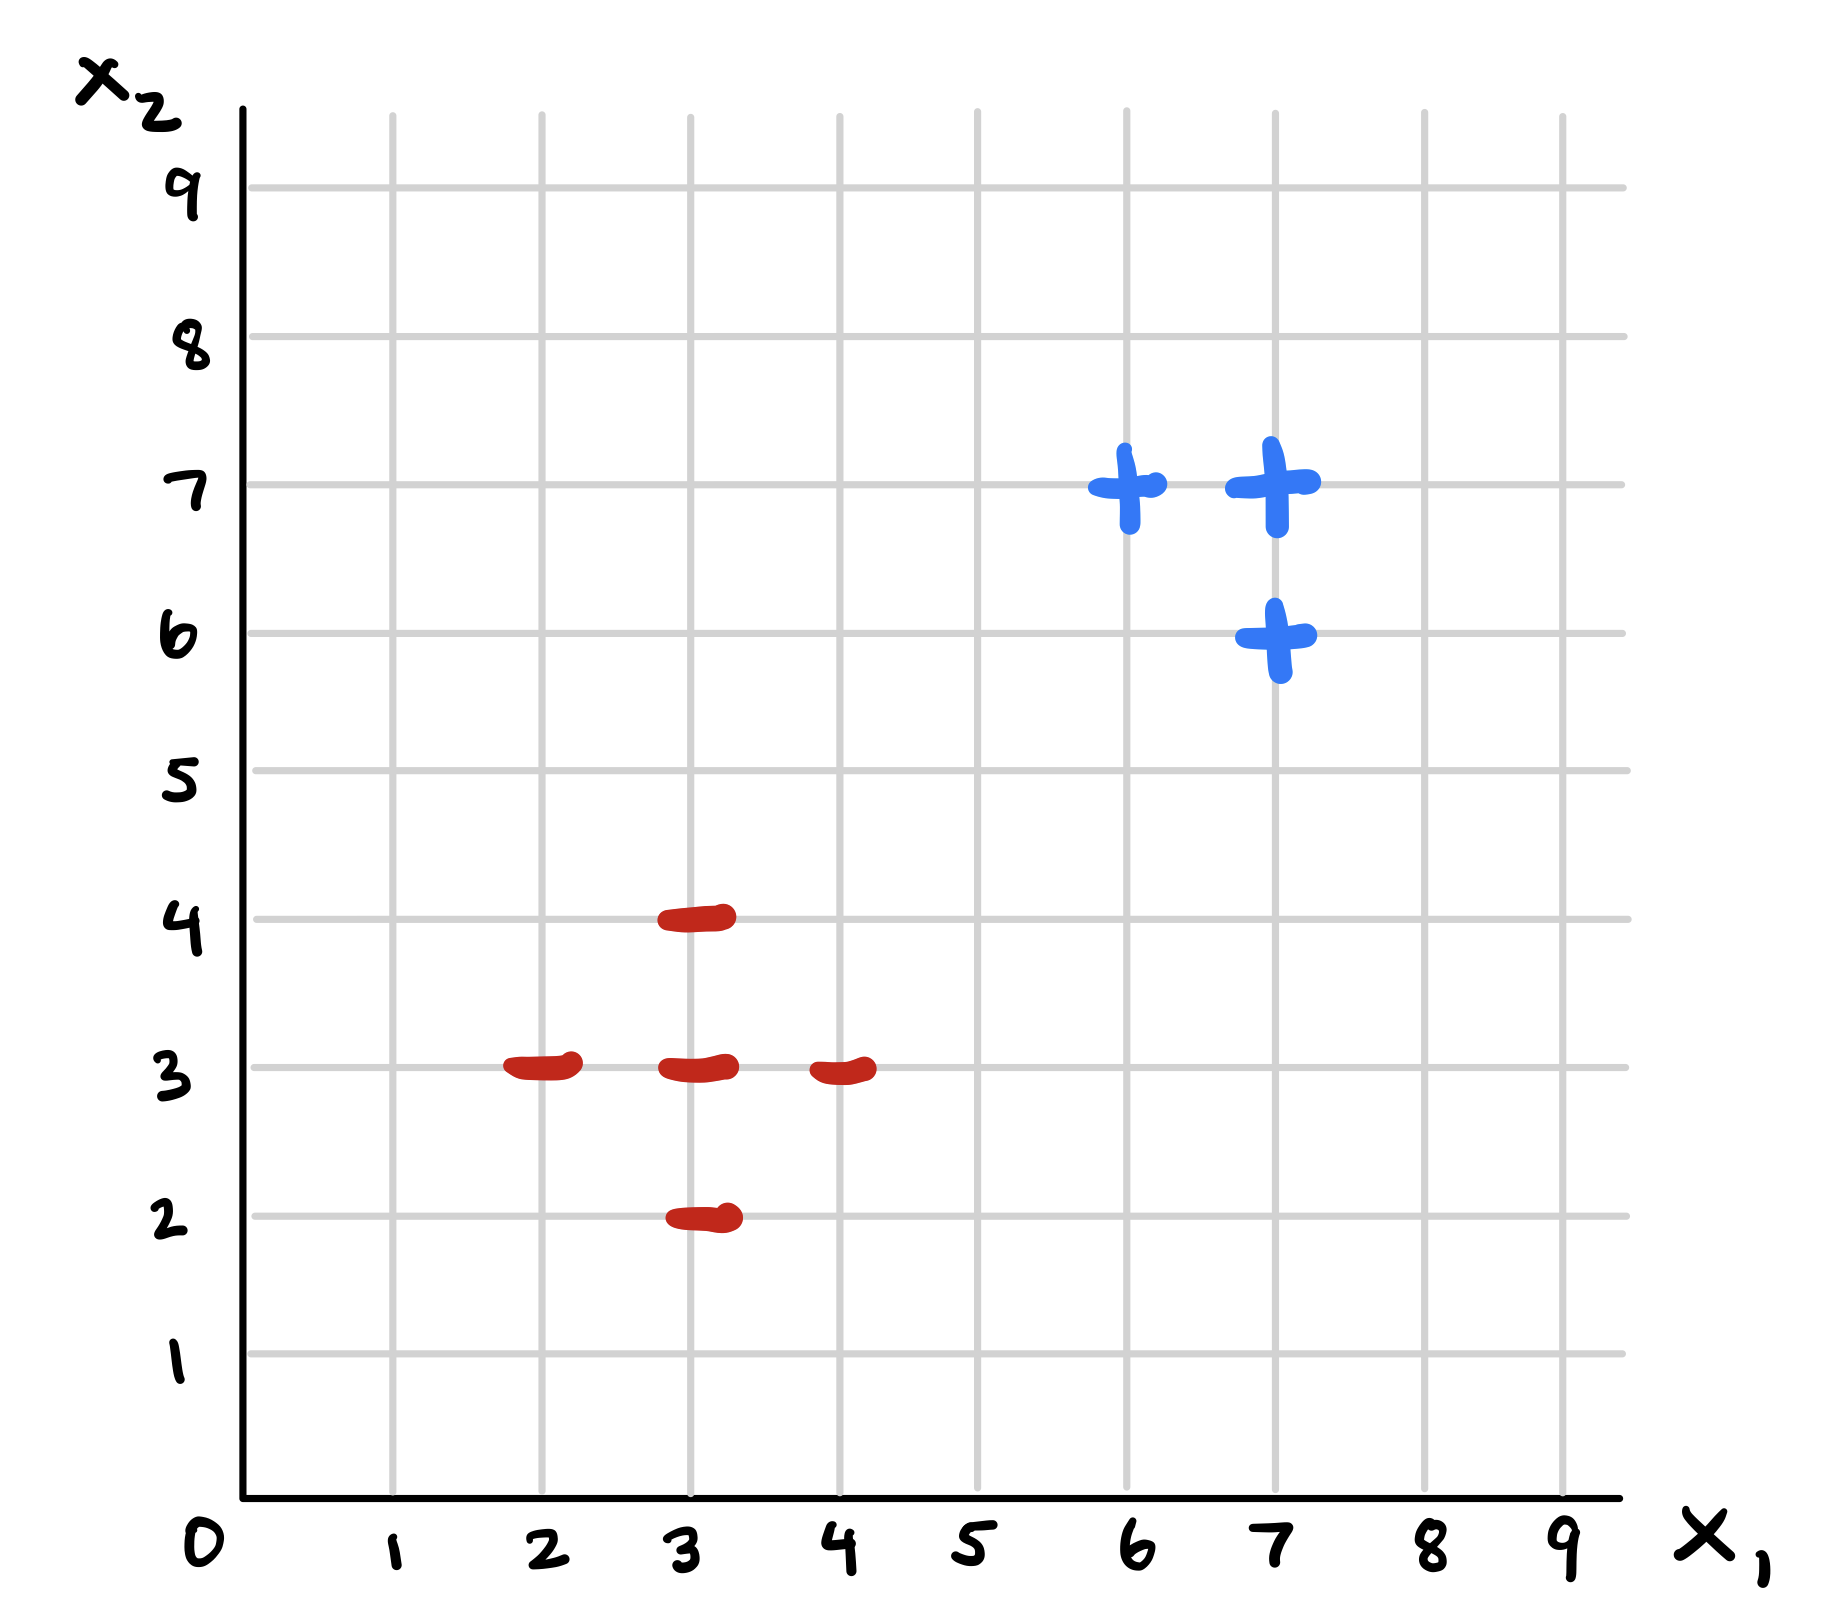
\includegraphics[scale=0.45]{exam2/figures/Exam2_S22_TA_mininet_dataset.png}
    
    Suppose we train each hidden unit individually by providing it with the corresponding feature $x_j$ and the label $y_i$ in the dataset above. Assume we use gradient descent on the negative log-likelihood.
    }

        \subpart[1]
            In the image above, draw the decision boundary learned by $v_1$. Label this boundary ``$v_1$''.

            \begin{soln}
                Any vertical line of the form $x_1=k$, where $k\in (4, 6)$
            \end{soln}


        \subpart[1]
            In the image above, draw the decision boundary learned by $v_2$. Label this boundary ``$v_2$''.

            \begin{soln}
                Any horizontal line of the form $x_2=k$, where $k\in (4, 6)$
            \end{soln} 
    
    
        \subpart[1]
            Name another ML model which can learn the same decision boundaries as Mininet's hidden units on this dataset.
            
            \begin{tcolorbox}[fit,height=3cm, width=15cm, blank, borderline={1pt}{-2pt}]
                % Solution goes here
            \end{tcolorbox}
            \begin{soln}
                Any classifier should be accepted as an answer, but targeting ``decision trees'' (Point of question: make connections between different ML models; test for understanding that logistic regression is a classifier)
            \end{soln}
            
        
        \subpart[2]
            Does each hidden unit \textit{individually} have a convex objective function?
            
            \begin{tcolorbox}[fit,height=3cm, width=15cm, blank, borderline={1pt}{-2pt}]
                % Solution goes here
            \end{tcolorbox}
            \begin{soln}
                Yes; the negative log-likelihood is convex.
            \end{soln}
    

    \uplevel{
    In the remaining questions, instead of training each hidden unit individually, we train the model as a whole using gradient descent on the negative log-likelihood.
    }
        \subpart[2]
            Does the model \textit{as a whole} have a convex objective function?
            
            \begin{tcolorbox}[fit,height=3cm, width=15cm, blank, borderline={1pt}{-2pt}]
                % Solution goes here
            \end{tcolorbox}
            \begin{soln}
                No; we can swap any two weights and biases and the corresponding elements of $\mathbf{w}_{out}$ to get the same solution (model is symmetric). (Point of question: test understanding about what makes a loss function non-convex in neural networks; I believe Matt also discussed this in lecture)
            \end{soln}


        \subpart[2]
            Given some loss function $J$, what is the gradient of the loss function with respect to $w_j$? That is, what is $\frac{\partial J}{\partial w_j}$? Leave your answer as the chain rule (i.e. as a product of partial derivatives). Do not skip any steps in the chain rule. \textit{You should not compute any derivatives for this question.}
            
            \begin{tcolorbox}[fit,height=3cm, width=15cm, blank, borderline={1pt}{-2pt}]
                % Solution goes here
            \end{tcolorbox}
            \begin{soln}
                $\frac{\partial J}{\partial \mathbf{z}_{out}}$
                $\frac{\partial \mathbf{z}_{out}}{\partial a_{out}}$
                $\frac{\partial a_{out}}{\partial z_i}$
                $\frac{\partial z_i}{\partial a_i}$
                $\frac{\partial a_i}{\partial w_i}$
            \end{soln}

    \uplevel{
    Now assume that each hidden unit uses a \textit{linear} activation function (i.e. $f$ is a linear function), but the output unit still uses the \textit{sigmoid} function (i.e. $g$ is the sigmoid function). Let's call this model Basic Mininet. Lamar Jackson, a huge fan of logistic regression, claims that a single logistic regression model is equivalent to Basic Mininet. In other words, he claims that a function is learnable by Basic Mininet if and only if it is learnable by a logistic regression model.
    }
        \subpart[2]
            Are there functions that Basic Mininet can learn but a logistic regression model cannot learn?
            
            \begin{tcolorbox}[fit,height=3cm, width=15cm, blank, borderline={1pt}{-2pt}]
                % Solution goes here
            \end{tcolorbox}
            \begin{soln}
                No; logistic regression can incorporate Basic Mininet's hidden layer implicitly, since composed linear functions are still linear.
            \end{soln}


        \subpart[2]
            Are there functions that a logistic regression model can learn but Basic Mininet cannot learn?
            
            \begin{tcolorbox}[fit,height=3cm, width=15cm, blank, borderline={1pt}{-2pt}]
                % Solution goes here
            \end{tcolorbox}
            \begin{soln}
                No; if each hidden unit computes the identity function, Basic Mininet is exactly the same as logistic regression.
            \end{soln}
            
            
        \subpart[2]
            Based on your above answers, is Lamar Jackson's claim correct?
            
            \begin{tcolorbox}[fit,height=3cm, width=15cm, blank, borderline={1pt}{-2pt}]
                % Solution goes here
            \end{tcolorbox}
            \begin{soln}
                Yes! (Point of this section: test understanding of model complexity and linear transformations; in lecture, Matt said that linear transformations of linear transformations are themselves linear, and this reasoning can be applied here)
            \end{soln}
    \end{subparts}
    
    
    \begin{qauthor}
       Chu. Learning objectives: Deep learning 1b: Combine simpler models (e.g. linear regression, binary logistic regression, multinomial logistic regression) as components to build up feed-forward neural network architectures
    \end{qauthor}


    \part[4] If we want to derive PAC bounds for \emph{regression} problems, we need to introduce the concept of \textbf{Pseudo-Dimension} and \textbf{P-Shattering}. For simplicity, we will consider the 1-dimensional case: consider a set of data $S = \{x^{(i)}\}_{i=1}^N$ and a hypothesis class $\mathcal{H}$ of regression functions. Now consider an arbitrary set of corresponding real-valued labels $\mathcal{Y} = \{y^{(i)}\}_{i=1}^N$ and the modified hypothesis space $\mathcal{H}'$ such that $\forall h \in \mathcal{H}$, we define each $h'$ as:
    $$h'(x^{(i)}) = \text{step}(h(x^{(i)}) - y^{(i)}),$$
    where $\text{step(x)} = 1$ if $x \ge 0$ and $0$ otherwise. Then $S$ is \emph{P-Shattered} by $\mathcal{H}$ if there exists some set $\mathcal{Y}$ such that $\mathcal{H}'$ shatters $S$. The \emph{Pseudo-Dimension} of $\mathcal{H}$ is the size of the largest set that is P-Shatterable by $\mathcal{H}$. This generalizes the notion of VC dimension for regression problems by discretizing the problem into "is the function above or below the current point" for every $x^{(i)}$.
 
    \begin{subparts}
        \subpart[2] Consider the hypothesis space $\mathcal{H}_1$ of y-axis centered positive parabolas (i.e. each $h \in \mathcal{H}_1$ is of the form $h(x) = ax^2 + c$ for some real $a, c$ and $a > 0$). Can $\mathcal{H}_1$ P-Shatter the following dataset? If so, provide an example of a labeling (as a list of each point and corresponding value) that $\mathcal{H}_1$ can capture. If not, briefly explain why.\\
        \begin{center}
            \begin{tikzpicture}[scale=2]
\draw[latex-latex] (-1.5,0) -- (2.5,0) ; %edit here for the axis
\foreach \x in  {-1,0,1,2} % edit here for the vertical lines
\draw[shift={(\x,0)},color=black] (0pt,3pt) -- (0pt,-3pt);
\foreach \x in {-1,0,1,2} % edit here for the numbers
\draw[shift={(\x,0)},color=black] (0pt,0pt) -- (0pt,-3pt) node[below] 
{$\x$};
\draw[o-o] (-1,0.0425);
\draw[o-o] (0,0.0425);
\draw[o-o] (2,0.0425);
\end{tikzpicture}
        \end{center}
        \usetikzlibrary{arrows}
    \fillwithlines{4em}
    \begin{soln}
        No. Since every parabola is centered at 0, there is no way for $h$ to be below the value at $x = 2$ without also always being below the value at $x = -1$.
    \end{soln}
    \subpart[2] Now consider the hypothesis space $\mathcal{H}_2$ of 1D 2-part piecewise linear functions (i.e. each $h$ represents a piecewise function of the form "if $x < c$ then $f(x)$ else $g(x)$" for some value $c$ and linear functions $f$ and $g$). What is the Pseudo-Dimension of $\mathcal{H}_2$?
    \begin{checkboxes}
        \choice 2
        \choice 3
        \choice 4
        \choice 5
    \end{checkboxes}
    \begin{soln}
        4
    \end{soln}
    \end{subparts}
    \begin{qauthor}
       Zack. Understanding VC dimension / shattering and synthesizing Learning Theory concepts with earlier regression material.
    \end{qauthor}
    
    
    
    \part[4]  
    Consider a coin flip (Bernoulli trial) with two possible outcomes. The probability of observing a Head (with value 1) is p, and the probability of observing a Tail (with value 0) is 1-p. 
    \begin{subparts}
        \subpart[1]
        What is the expected value for one trial of coin flip? \\
        \begin{tcolorbox}[fit,height=1cm, width=15cm, blank, borderline={1pt}{-2pt}]
        %solution
        \end{tcolorbox}
        \begin{soln}
        $1\times p + 0\times (1-p) = p$
        \end{soln}
        
        \subpart[1]
        Derive the variance for one trial of coin flip.
        \begin{tcolorbox}[fit,height=2cm, width=15cm, blank, borderline={1pt}{-2pt}]
        %solution
        \end{tcolorbox}
        \begin{soln}
        $Var[X] = E[X^2]-E[X]^2 = \sum_{x=0,1} x^2p(x) - p^2 = p - p^2 = p(1-p)$
        \end{soln}
        
        \subpart[1]
        Recall that Binomial Distribution represents n independent Bernoulli trials. Consider tossing this same coin n times. What is the expected value now?
         \begin{tcolorbox}[fit,height=2cm, width=15cm, blank, borderline={1pt}{-2pt}]
        %solution
        \end{tcolorbox}
        \begin{soln}
        $E[X_1+X_2+...X_n] = E[X_1]+E[X_2]+...+E[X_n] = n*p $ due to independence
        \end{soln}
        
        \subpart[1]
        Derive the variance of n trials of coin flips.
        \begin{tcolorbox}[fit,height=2cm, width=15cm, blank, borderline={1pt}{-2pt}]
        %solution
        \end{tcolorbox}
        \begin{soln}
        $Var(\sum_{i=1}^{m} X_i) = \sum_{i=1}^{m} Var(X_i) + 2 \sum_{i<j} Cov(X_i,X_j) $ \\
        $ = \sum_{i=1}^{m} Var(X_i)$ due to independence\\
        $ = np(1-p)$
        \end{soln}
        
    \end{subparts}
    \begin{qauthor}
    Yuxin. MLE and MAP (a). Expected value, variance and independence.
    
    \end{qauthor}
    
    

    
    \part Suppose $x_{1}, \ldots, x_{n}$ are independent and identically distributed samples from a distribution with density
$$
f_{X}(x \mid \theta)=\left\{\begin{array}{cl}
\frac{\theta x^{\theta-1}}{3^{\theta}}, & 0 \leq x \leq 3 \\
0, & \text { otherwise }
\end{array}\right.
$$
Find the MLE for $\theta$.
\begin{tcolorbox}[fit,height=2cm, width=15cm, blank, borderline={1pt}{-2pt}]
        %solution
        \end{tcolorbox}
        
    \begin{soln}

    $$
\begin{aligned}
L\left(x_{1}, \ldots, x_{n} \mid \theta\right) &=\prod_{i=1}^{n} \frac{\theta x_{i}^{\theta-1}}{3^{\theta}} \\
\ln L\left(x_{1}, \ldots, x_{n} \mid \theta\right) &=\sum_{i=1}^{n}\left(\ln \theta+(\theta-1) \ln x_{i}-\theta \ln 3\right) \\
\frac{\partial}{\partial \theta} \ln L\left(x_{1}, \ldots, x_{n} \mid \theta\right) &=\sum_{i=1}^{n}\left(\frac{1}{\theta}+\ln x_{i}-\ln 3\right)=0 \\
\frac{n}{\hat{\theta}}+\sum_{i=1}^{n} \ln x_{i}-n \ln 3 &=0 \\
\frac{n}{\hat{\theta}} &=n \ln 3-\sum_{i=1}^{n} \ln x_{i} \\
\hat{\theta}_{\mathrm{MLE}} &=\frac{n}{n \ln 3-\sum_{i=1}^{n} \ln x_{i}}
\end{aligned}
$$
Check that it is a maximum by showing the second derivative is negative for all values of $\theta$.
$$
\frac{\partial^{2}}{\partial \theta^{2}} \ln L\left(x_{1}, \ldots, x_{n} \mid \theta\right)=\sum_{i=1}^{n}\left(-\frac{1}{\theta^{2}}\right)=-\frac{n}{\theta^{2}}<0
$$
so $\ln L\left(x_{1}, \ldots, x_{n} \mid \theta\right)$ is concave downward everywhere.
    \end{soln}
    
    \begin{qauthor}
    Junhui, Derive MLE formula given density function of specific distribution.

    \end{qauthor}
    
    
    
\end{parts}



    





